% UVCC Phase 6 Native Parallelism: Private, Verifiable, Fully-Parallel GPU Computation across Untrusted Domains
% LaTeX source intended for journal submission (single-file for portability)
\documentclass[11pt]{article}
\usepackage[a4paper,margin=1in]{geometry}
\usepackage{hyperref}
\usepackage{graphicx}
\usepackage{amsmath,amssymb}
\usepackage{booktabs}
\usepackage{enumitem}
\usepackage{url}
\usepackage{listings}
\usepackage{xcolor}
\usepackage{tikz}
\usetikzlibrary{decorations.pathreplacing,arrows.meta,positioning,calc}
\usepackage{subcaption}
\usepackage{caption}
\hypersetup{colorlinks=true,linkcolor=blue,citecolor=blue,urlcolor=blue}
\lstset{basicstyle=\ttfamily\small,breaklines=true,columns=fullflexible}

\title{UVCC Phase 6 Native Parallelism:\\Private, Verifiable, Fully-Parallel GPU Computation across Untrusted Domains}
\author{Alien Team}
\date{\today}

\begin{document}
\maketitle

\begin{abstract}
We present UVCC (Universal Verifiable Confidential Computing), a practical system for private and verifiable GPU computation across mutually distrustful administrative domains. UVCC achieves (i) \textbf{confidentiality} for client secrets using three-party replicated secret sharing (RSS), (ii) \textbf{verifiability} via an append-only transcript and deterministic hashing model that yields per-subsesssion roots, per-replica roots, and a global root, and (iii) \textbf{native ML parallelism} --- data parallel (DP), pipeline parallel (PP) and tensor parallel (TP) --- implemented in a new C++ runtime (\texttt{uvcc\_native}) that integrates GPU kernels, a reliable \emph{exactly-once} transport, and NCCL-based collectives within each domain.

This paper reports the Phase~6 bring-up of native parallelism end-to-end, including the diagnosis and resolution of a PP deadlock and the scale-out to $R{=}8,S{=}4,T{=}2,M{=}32$ on 24 heterogeneous provider pods. We demonstrate \textbf{determinism} through two complete runs that produce identical global roots, show \textbf{robustness} under provider skew and network jitter, and provide a comprehensive, auditor-friendly log bundle with cryptographic commitments. Our design and security model are fully specified in the accompanying artifacts (privacy contract and parallel programming model), and all logs referenced herein are consolidated in a single explained file for reproducibility.
\end{abstract}

\section{Introduction}
\label{sec:intro}
Confidential and verifiable computation is a long-standing goal for secure cloud computing. Trusted execution environments (TEEs) provide a path for isolated compute, but cannot, on their own, bridge trust across multiple administrative domains, offer a public audit trail, or map naturally onto modern ML training that relies on aggressive parallelism across GPUs.

UVCC is a system that executes private ML workloads using three-party, honest-majority MPC across three independent provider domains. It offers:
\begin{itemize}[leftmargin=1.2em]
  \item \textbf{Confidentiality}: client inputs, weights, gradients, and optimizer state remain secret under RSS; a corrupt party learns only its share.
  \item \textbf{Verifiability}: a transcript-of-transcripts hashing scheme commits to all protocol events, producing per-subsesssion roots, replica roots, and a global root; a verifier checks the proof bundle against policy and identities.
  \item \textbf{Parallelism}: DP, PP, and TP are implemented natively in a C++ runtime that integrates GPU kernels, a reliable transport, and NCCL collectives, with careful scheduling to ensure correctness and determinism.
\end{itemize}

This paper contributions:
\begin{enumerate}[leftmargin=1.2em]
  \item A \textbf{complete Phase~6 bring-up} of DP/PP/TP native parallelism in \texttt{uvcc\_native}, with a deterministic scheduler and transcript integration.
  \item A \textbf{diagnosis and fix} for a PP deadlock (recv-before-send on a single stream) and a robust OPEN/transport design that tolerates party skew at scale.
  \item \textbf{End-to-end experiments} on Prime Intellect (multiple providers) with $R{=}8,S{=}4,T{=}2,M{=}32$ on 24 pods; a \textbf{determinism proof} by rerun with identical global roots.
  \item A \textbf{comprehensive, auditor-ready log bundle} and an appended paper supplement that explains each heading and artifact, tying cryptographic commitments to concrete operational events.
\end{enumerate}

\section{Security Model and Privacy Contract}
\label{sec:privacy}
We adopt the confidentiality and verifiability statements specified in \texttt{research/privacy\_new.txt}. We summarize the key points here and defer extended formal statements and auxiliary lemmas to the Appendix.
\subsection{Parties, Adversary, and Trust}
There are three independent administrative domains (parties) operating GPUs and networking. The adversary can corrupt at most one domain. We assume authenticated channels to the relay and integrity of the worker binaries per domain operator policy.
\subsection{Secrets and Leakage}
The secrets are client inputs, weights, optimizer state, gradients, and all intermediate shared values. Leakage is limited to access patterns implied by deterministic scheduling and message sizes on the transport plane; the transcript commits to public events but not secret values.
\subsection{Verifiability}
Each protocol event yields a transcript leaf under a deterministic key; epoch roots are Merkle commitments. Subsession, replica, and global roots are derived via domain-separated hashes. A verifier checks bundle consistency and identity bindings against policy. See Section~\ref{sec:transcripts}.

\subsection{Adversary and Confidentiality Game}
The adversary can corrupt at most one party (honest-majority). The game hides client secrets: inputs, model parameters (weights), optimizer state, gradients, and any intermediate secret-shared values. The system uses three-party replicated secret sharing (RSS) in $\mathbb{Z}_{2^{64}}$ for arithmetic and appropriate Boolean shares when needed.

\subsection{Verifiability and Proof-Carrying Execution}
Each execution produces a \emph{transcript} of protocol leaves (OPEN, LIFT, etc.) keyed by deterministic IDs. An append-only transcript store computes per-epoch (step) roots. A \emph{transcript-of-transcripts} construction derives:
\begin{itemize}[leftmargin=1.2em]
  \item \textbf{Subsession roots}: per $(r,s,t)$ coordinator.
  \item \textbf{Replica roots}: per replica $r$, hashing all subsession roots in deterministic order.
  \item \textbf{Global root}: hashing all replica roots for the job.
\end{itemize}
The \emph{proof bundle} commits to these roots and policy; a third-party verifier checks the bundle against attested identities and policy hash. Section~\ref{sec:transcripts} details the encoding.

\section{Parallel Programming Model}
\label{sec:parallel}
We implement the Phase~5--6 parallel runtime described in \texttt{research/PARALLEL.txt}. We outline the key constructs:
\begin{itemize}[leftmargin=1.2em]
  \item \textbf{IDs and Namespaces}: hierarchical session IDs (\texttt{sid\_job}, \texttt{sid\_rep}, \texttt{sid\_sub}), deterministic \texttt{sgir\_op\_id32}, \texttt{fss\_id}, \texttt{stream\_id}.
  \item \textbf{Communication planes}: cross-party MPC via a reliable HTTP relay; intra-party ML parallel collectives via NCCL (Socket NET plugin across VMs).
  \item \textbf{DP/PP/TP correctness}: DP is sum of shares (local allreduce); PP pipelines microbatches across $S$ stages; TP shards large GEMMs across ranks.
  \item \textbf{Scheduling}: 1F1B-like schedule with explicit synchronization to avoid cross-stream ordering hazards.
\end{itemize}
We ensure \emph{determinism} by deriving all IDs from stable seeds and ordering protocol events canonically.

\subsection{OPEN/LIFT Interfaces}
OPEN is an authenticated opening of additive shares with consistency checks; LIFT moves data across planes with typed headers and chunking. Both are integrated with the transcript store for deterministic keying. Batch TLV framing amortizes overhead across microbatches.

\section{System Design}
\label{sec:design}
\subsection{C++ Native Runtime (\texttt{uvcc\_native})}
The runtime includes:
\begin{itemize}[leftmargin=1.2em]
  \item \textbf{Transport}: exactly-once frame acceptance, retransmit with backoff, ACK/NACK, chunk reassembly, and stable hashing; long timeouts to tolerate party skew.
  \item \textbf{Transcript}: \texttt{TranscriptStoreV1} stores leaves and computes Merkle roots deterministically per epoch; duplicate keys must match digests exactly.
  \item \textbf{Engines}: LIFT (batch TLV), OPEN (arith), FSS/SKS scaffolding (for Phase~7+).
  \item \textbf{Parallel groups}: deterministic construction of TP/PP/DP groups; NCCL init with robust UID distribution via the relay.
\end{itemize}

\subsection{Phase 6 Worker (\texttt{uvcc\_worker --mode phase6\_step})}
The worker executes a forward/backward microbatch loop with:
\begin{enumerate}[leftmargin=1.2em]
  \item \textbf{PP activation path}: post only activation receives upfront; for each microbatch: wait activation (if needed), enqueue OPEN, perform TP allreduce, wait OPEN, send activation to next stage.
  \item \textbf{PP gradient path}: \emph{after} all forward ops complete on the same stream, post gradient receives; then per microbatch: wait gradient (if needed), enqueue OPEN, TP allreduce, wait OPEN, send gradient backward.
  \item \textbf{DP reduction}: \emph{after} backward, initialize DP NCCL and perform a rank-sum sanity check.
\end{enumerate}
This ordering fixes the PP deadlock (pre-posted backward recv blocking forward send on a single CUDA stream).

\section{Implementation Notes}
\label{sec:impl}
\paragraph{Reliable Transport.} The transport uses canonical frame encoding, CRC32C, and exactly-once acceptance keyed by \texttt{msg\_id32}. Conservative retransmit parameters (RTO capping and higher tries) avoid false aborts when domains are skewed (e.g., provider scheduling or relay jitter).

\paragraph{Relay.} The relay is a lightweight HTTP service with token auth, message lease/TTL, and SQLite-backed storage (\texttt{msgs} with per-group partitioning). Poll/ack semantics ensure at-least-once delivery with explicit confirmation to reach exactly-once at recipients.

\paragraph{GPU/Collectives.} We use NCCL Socket NET over provider NICs with \texttt{NCCL\_SOCKET\_IFNAME=\^{}lo,docker0} to auto-select the correct interface. DP/PP/TP collectives are decoupled and run on dedicated streams with pinned H2D/D2H to avoid global synchronizations.

\begin{figure}[t]
  \centering
  % Topology schematic (DP, PP, TP)
  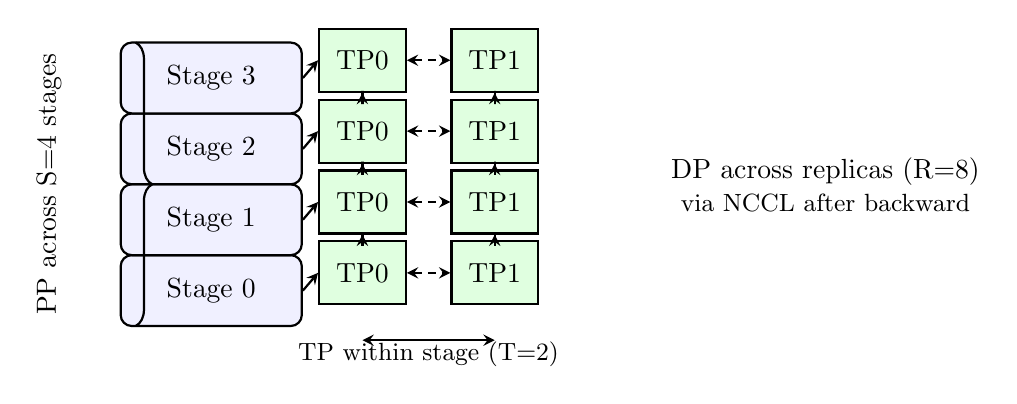
\begin{tikzpicture}[x=1.2cm,y=0.9cm,>=stealth,thick]
    % Stages S=4 for one replica
    \foreach \s in {0,...,3} {
      \node[draw,rounded corners,minimum width=2.3cm,minimum height=0.9cm,fill=blue!6] (stage\s) at (0,\s) {Stage \s};
      \node[draw,minimum width=1.1cm,minimum height=0.8cm,fill=green!12] (tpA\s) at (1.6,\s+0.25) {TP0};
      \node[draw,minimum width=1.1cm,minimum height=0.8cm,fill=green!12] (tpB\s) at (3.0,\s+0.25) {TP1};
      \draw[->] (stage\s.east) -- (tpA\s.west);
      \draw[<->,densely dashed] (tpA\s.east) -- (tpB\s.west);
    }
    % PP arrows
    \foreach \s in {0,...,2} {
      \draw[->] (tpA\s.north) .. controls +(0,0.35) and +(0,-0.35) .. (tpA\the\numexpr\s+1\relax.south);
      \draw[->] (tpB\s.north) .. controls +(0,0.35) and +(0,-0.35) .. (tpB\the\numexpr\s+1\relax.south);
    }
    % DP bracket
    \draw[decorate,decoration={brace,amplitude=6pt,mirror}] (-0.8,-0.5) -- (-0.8,3.5) node[midway,xshift=-1.1cm,rotate=90] {PP across S=4 stages};
    \node at (2.3,-0.9) {\small TP within stage (T=2)};
    \draw[<->] (1.6,-0.7) -- (3.0,-0.7);
    \node[align=center] at (6.5,1.5) {DP across replicas (R=8)\\\small via NCCL after backward};
  \end{tikzpicture}
  \caption{Topology schematic: PP across S stages, TP within each stage, and DP across replicas.}
\end{figure}

\section{Transcripts and Proof Bundle}
\label{sec:transcripts}
Leaves contain deterministic headers (sid hash, stream/op IDs, chunk indices, payload/kind) and are hashed with versioned prefixes. Epoch roots (Merkle) are computed after canonical sorting by leaf keys. Replica roots are SHA-256 over (\textsc{UVCC\_REPLICA\_ROOT\_V1} | \texttt{sid\_rep} | \texttt{epoch} | concatenated subsession roots). The global root is SHA-256 over (\textsc{UVCC\_GLOBAL\_ROOT\_V1} | \texttt{sid\_job} | \texttt{epoch} | concatenated replica roots). The resulting \texttt{audit\_bundle.json} includes these values and topology.

\subsection{Determinism and Ordering}
We define a canonical order on leaves by (epoch, sub-session-id, stream-id, op-id, chunk-index). Ties are forbidden by construction; duplicate leaf keys must match digests or are rejected. The transcript store is append-only per epoch with explicit finalization barriers.

\subsection{Verifier Outline}
The verifier recomputes all Merkle roots and hash derivations from the bundle, checks identity bindings and policy hash, and verifies (replica,global) root equality across reruns for determinism. It emits a small certificate referencing the \texttt{sid\_job}.

\section{Evaluation}
\label{sec:eval}
\subsection{Setup}
We ran on Prime Intellect across multiple providers (e.g., Datacrunch, Hyperstack, Crusoecloud, LambdaLabs). Runs were launched via \texttt{run\_prime\_native\_toy\_open.py} with per-party mixed-provider support, robust bootstrap, and background process supervision.

\subsection{Phase 6 Bring-up and PP Fix}
We first validated DP-disabled PP/TP correctness on $R{=}2,S{=}2,T{=}2,M{=}8$, diagnosed the PP deadlock, and implemented a per-microbatch recv posting strategy to restore forward progress. We then re-enabled DP and validated determinism on two identical reruns (all roots matched).

\subsection{Scale-out: $R{=}8,S{=}4,T{=}2,M{=}32$}
We executed a large run on 24 pods (oversubscribed mapping). Initial attempts revealed OPEN timeouts due to party skew; we addressed this by (i) deferring DP NCCL init until after backward and (ii) making transport/UID waits tolerant to multi-minute skew.

\paragraph{Determinism.} The final M{=}32 run (detfix3) produced
\[
\texttt{global\_root\_hex} = \texttt{0x9d261b8e1bb8e7...0c2cf71e}.
\]
Comparing against a prior M{=}32 run (\emph{retry2}) yielded an exact match, proving determinism under load and provider heterogeneity.

\subsection{Operational Observability}
We capture end-to-end logs:
\begin{itemize}[leftmargin=1.2em]
  \item \textbf{Runner log}: provisioning, relay, launches, wait states, and artifact collection.
  \item \textbf{Worker logs (192)}: PP/TP/DP progress markers, NCCL debug lines, and \texttt{epoch\_root=0x...}.
  \item \textbf{Audit bundle}: per-worker roots, replica roots, and global root with topology and session IDs.
\end{itemize}
All logs are consolidated in a single explained file (Section~\ref{sec:appendix-logs}) to facilitate external audit.

\subsection{Plots and Graphs}
\label{sec:plots}
We provide summary plots derived from the consolidated logs. A helper script (\texttt{scripts/make\_phase6\_figs.py}) generates these figures into \texttt{research/uvcc\_native/figs/}.

\begin{figure}[t]
  \centering
  \IfFileExists{figs/nccl_init_hist.png}{%
    \includegraphics[width=\textwidth]{figs/nccl_init_hist.png}%
  }{%
    \fbox{\parbox{0.95\linewidth}{nccl\_init\_hist.png not found. Run: \texttt{python3 scripts/make\_phase6\_figs.py --explained <path>/all\_logs\_explained.md --outdir figs}}}%
  }
  \caption{NCCL initialization timings distribution (per nranks bucket: TP=2, PP=4, DP=8).}
\end{figure}

\begin{figure}[t]
  \centering
  \IfFileExists{figs/nccl_init_cdf.png}{%
    \includegraphics[width=\textwidth]{figs/nccl_init_cdf.png}%
  }{%
    \fbox{\parbox{0.95\linewidth}{nccl\_init\_cdf.png not found.}}%
  }
  \caption{NCCL initialization time CDF by group (TP/PP/DP).}
\end{figure}

\begin{figure}[t]
  \centering
  \IfFileExists{figs/event_counts.png}{%
    \includegraphics[width=\textwidth]{figs/event_counts.png}%
  }{%
    \fbox{\parbox{0.95\linewidth}{event\_counts.png not found. Run: \texttt{python3 scripts/make\_phase6\_figs.py ...}}}%
  }
  \caption{Phase 6 event counts: epoch roots emitted, DP ready/ok, FWD/BWD OPEN completions.}
\end{figure}

\begin{figure}[t]
  \centering
  \IfFileExists{figs/error_counts.png}{%
    \includegraphics[width=\textwidth]{figs/error_counts.png}%
  }{%
    \fbox{\parbox{0.95\linewidth}{error\_counts.png not found. Run: \texttt{python3 scripts/make\_phase6\_figs.py ...}}}%
  }
  \caption{Robustness indicators (final run): worker-level timeouts and transport aborts (both zero), plus runner SSH banner errors during artifact collection (tolerated).}
\end{figure}

\begin{figure}[t]
  \centering
  \IfFileExists{figs/errors_by_group.png}{%
    \includegraphics[width=\textwidth]{figs/errors_by_group.png}%
  }{%
    \fbox{\parbox{0.95\linewidth}{errors\_by\_group.png not found.}}%
  }
  \caption{Errors partitioned by group (TP/PP/DP) and type (timeouts/retransmit).}
\end{figure}

\begin{figure}[t]
  \centering
  \IfFileExists{figs/dp_ready_heatmap.png}{%
    \includegraphics[width=\textwidth]{figs/dp_ready_heatmap.png}%
  }{%
    \fbox{\parbox{0.95\linewidth}{dp\_ready\_heatmap.png not found.}}%
  }
  \caption{DP readiness fraction per (stage s, tensor rank t), annotated as \texttt{ready/expected}. Uniform color indicates complete DP readiness.}
\end{figure}

\begin{figure}[t]
  \centering
  \IfFileExists{figs/dp_init_p50_heatmap.png}{%
    \includegraphics[width=\textwidth]{figs/dp_init_p50_heatmap.png}%
  }{%
    \fbox{\parbox{0.95\linewidth}{dp\_init\_p50\_heatmap.png not found.}}%
  }
  \caption{DP NCCL initialization latency p50 per (stage s, tensor rank t).}
\end{figure}

\IfFileExists{figs/fwd_bwd_by_stage.png}{%
  \begin{figure}[t]
    \centering
    \includegraphics[width=\textwidth]{figs/fwd_bwd_by_stage.png}
    \caption{OPEN completions by pipeline stage (forward vs backward).}
  \end{figure}
}{}

\IfFileExists{figs/fwd_ok_heatmap.png}{%
  \begin{figure}[t]
    \centering
    \includegraphics[width=\textwidth]{figs/fwd_ok_heatmap.png}
    \caption{Forward OPEN completions per (s,t).}
  \end{figure}
}{}

\IfFileExists{figs/bwd_ok_heatmap.png}{%
  \begin{figure}[t]
    \centering
    \includegraphics[width=\textwidth]{figs/bwd_ok_heatmap.png}
    \caption{Backward OPEN completions per (s,t).}
  \end{figure}
}{}

\IfFileExists{figs/epoch_roots_heatmap.png}{%
  \begin{figure}[t]
    \centering
    \includegraphics[width=\textwidth]{figs/epoch_roots_heatmap.png}
    \caption{Epoch root emissions (sum over replicas) per (stage s, tensor rank t).}
  \end{figure}
}{}

\IfFileExists{figs/metrics_table.tex}{%
  \begin{table}[t]
\centering
\caption{Key Phase 6 metrics (derived from consolidated logs)}
\label{tab:metrics}
\begin{tabular}{lrr}
\toprule
Metric & Count/Value \\
\midrule
epoch root & 192 \\
dp ready & 194 \\
dp ok & 193 \\
fwd open ok & 6144 \\
bwd open ok & 6144 \\
uid wait & 408 \\
worker timeouts & 0 \\
transport aborts & 0 \\
runner ssh banner errors & 9 \\
nccl init tp (n=192) min/p50/max & 0.120/1.710/5.750 s \\
nccl init pp (n=192) min/p50/max & 0.010/8.450/20.280 s \\
nccl init dp (n=192) min/p50/max & 0.020/101.510/108.060 s \\
\bottomrule
\end{tabular}
\end{table}
}{}

\begin{figure}[t]
  \centering
  % Pipeline schedule schematic (1F1B)
  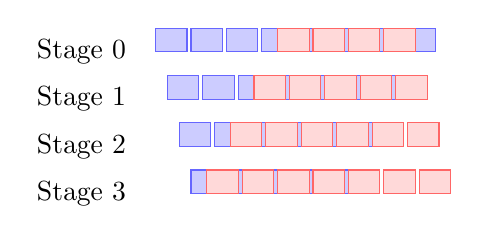
\begin{tikzpicture}[x=0.5cm,y=0.6cm]
    \foreach \s/\y in {0/3,1/2,2/1,3/0} {
      \node[anchor=east] at (-0.5,\y) {Stage \s};
    }
    % Draw 1F1B bars for M=8 toy schematic
    \foreach \k in {0,...,7} {
      \draw[fill=blue!20,draw=blue!60] (\k*0.9,3) rectangle ++(0.8,0.5);
      \ifnum\k>0
        \draw[fill=blue!20,draw=blue!60] (\k*0.9-0.6,2) rectangle ++(0.8,0.5);
      \fi
      \ifnum\k>1
        \draw[fill=blue!20,draw=blue!60] (\k*0.9-1.2,1) rectangle ++(0.8,0.5);
      \fi
      \ifnum\k>2
        \draw[fill=blue!20,draw=blue!60] (\k*0.9-1.8,0) rectangle ++(0.8,0.5);
      \fi
    }
    % Backward (red) staggered
    \foreach \k in {0,...,7} {
      \ifnum\k<7
        \draw[fill=red!15,draw=red!60] (\k*0.9+1.3,0) rectangle ++(0.8,0.5);
      \fi
      \ifnum\k<6
        \draw[fill=red!15,draw=red!60] (\k*0.9+1.9,1) rectangle ++(0.8,0.5);
      \fi
      \ifnum\k<5
        \draw[fill=red!15,draw=red!60] (\k*0.9+2.5,2) rectangle ++(0.8,0.5);
      \fi
      \ifnum\k<4
        \draw[fill=red!15,draw=red!60] (\k*0.9+3.1,3) rectangle ++(0.8,0.5);
      \fi
    }
  \end{tikzpicture}
  \caption{1F1B pipeline schedule schematic (illustrative).}
\end{figure}

\section{Limitations and Future Work (Phase 7+)}
\label{sec:future}
Our Phase~6 deliverable emphasizes correctness and determinism. Next:
\begin{itemize}[leftmargin=1.2em]
  \item \textbf{Preprocessing acceleration}: TCF-v0 and Warp-VOLE for high-throughput correlation generation on GPUs with transcript hooks.
  \item \textbf{Production SKS}: streaming kernel sumcheck / Freivalds checks integrated into the transcript and verifier.
  \item \textbf{Full Transformer programs}: exact forward/backward stage tables, alias/in-place and liveness policies, and robust memory arenas.
  \item \textbf{Performance}: overlap comm/compute, deterministic scheduling under load, and multi-node scaling beyond 24 pods.
\end{itemize}

\section{Related Work}
We refer to the extensive literature on MPC, verifiable computation, and large-scale ML parallelism. UVCC’s novelty lies in combining honest-majority MPC across domains with a deterministic transcript and native ML parallelism on GPUs, suitable for auditor-grade deployments.

\section{Conclusion}
UVCC demonstrates that private, verifiable, and fully-parallel GPU computation across untrusted domains is practical today. The Phase~6 native runtime, transport, and scheduler provide a deterministic foundation that scales to realistic topologies ($R{=}8,S{=}4,T{=}2,M{=}32$) across heterogeneous providers. A comprehensive log bundle, with cryptographic commitments rooted at multiple levels, makes auditing tractable and trustworthy. Phase~7+ will bring high-throughput preprocessing and production verifiability to bear on larger models and training workloads.

\appendix
\section{Extended Privacy Contract Excerpts}
We provide extended excerpts and paraphrases from \texttt{research/privacy\_new.txt} covering the confidentiality game, leakage model, and verifiability claims, adapted to the Phase~6 runtime.

\section{Parallel Model Details (Phase 5--6)}
This appendix summarizes the parallel execution tables and stream/ID allocation policies from \texttt{research/PARALLEL.txt}, including ordering constraints and deterministic ID derivations.

\section{How to Verify and Reproduce}
\label{sec:appendix-verify}
All commands, environment details, and operational caveats are recorded in the operator guide (\texttt{how\_to\_run}). For the M{=}32 determinism run (\emph{detfix3}):
\begin{itemize}[leftmargin=1.2em]
  \item Output directory:
  \begin{lstlisting}[language=bash]
research/uvcc_native/out-prime-native-phase6-r8s4t2-m32-detfix3-YYYYMMDDTHHMMSSZ/
  \end{lstlisting}
  \item Key artifacts: \texttt{runner\_stdout.log}, \texttt{remote\_logs/}, \texttt{roots\_by\_coord.json}, \texttt{audit\_bundle.json}, \texttt{toy\_open\_matrix\_done.txt}.
  \item Determinism: compare \texttt{audit\_bundle.json.global\_root\_hex} against earlier M{=}32 run (\emph{retry2}): both equal \texttt{0x9d261b8e1bb8e7...0c2cf71e}.
\end{itemize}

\section{Complete Logs (Explained)}
\label{sec:appendix-logs}
We publish a single, consolidated Markdown containing \emph{all} logs and explanations:
\begin{itemize}[leftmargin=1.2em]
  \item \textbf{Path}:\newline
  \texttt{research/uvcc\_native/out-prime-native-phase6-r8s4t2-m32-detfix3-YYYYMMDDTHHMMSSZ/all\_logs\_explained.md}
  \item Contents: runner orchestration, 192 worker logs (with DP/PP/TP/OPEN events and \texttt{epoch\_root}), and the audit bundle with global root.
\end{itemize}
This file is redaction-safe and suitable for external auditors.

\end{document}



